%%%%%%%%%%%%%%%%%%%%%%%%% Shortest Paths %%%%%%%%%%%%%%%%%%%%%%%%%%

\section{Shortest Paths}

\begin{frame}
  \frametitle{Shortest paths}

  \textcolor{purple}{Different editions of shortest paths problems:}
  \begin{enumerate}
    \item shortest(longest) path in DAG  \\
      \emph{\textcolor{blue}{Dynamic Programming}}
    \item single-source shortest paths
      \begin{itemize}
        \item No negative edges. \\
          \emph{\textcolor{blue}{Dijkstra algorithm.}}
        \item With negative edges (No negative cycle). \\
          \emph{\textcolor{gray}{Bellman-Ford algorithm.}}
      \end{itemize}
    \item all pairs shortest paths \\
      \emph{\textcolor{blue}{Floyd-Warshall algorithm.}}
  \end{enumerate}

\end{frame}

%\begin{frame}
%  \frametitle{Shortest paths}
%
%  \textcolor{purple}{To better understand these problems and algorithms:}
%  \vspace{0.40cm}
%
%  \begin{enumerate}
%    \setlength{\itemsep}{0.30cm}
%    \item Why the algorithm works for this problem ?
%    \item Does the algorithm also work for another problem ?
%  \end{enumerate}
%
%\end{frame}


\begin{frame}
  \frametitle{Shortest paths}

  \textcolor{purple}{DAG can be topologically sorted, so \emph{DP} works.}

  \begin{figure}
    \begin{center}
      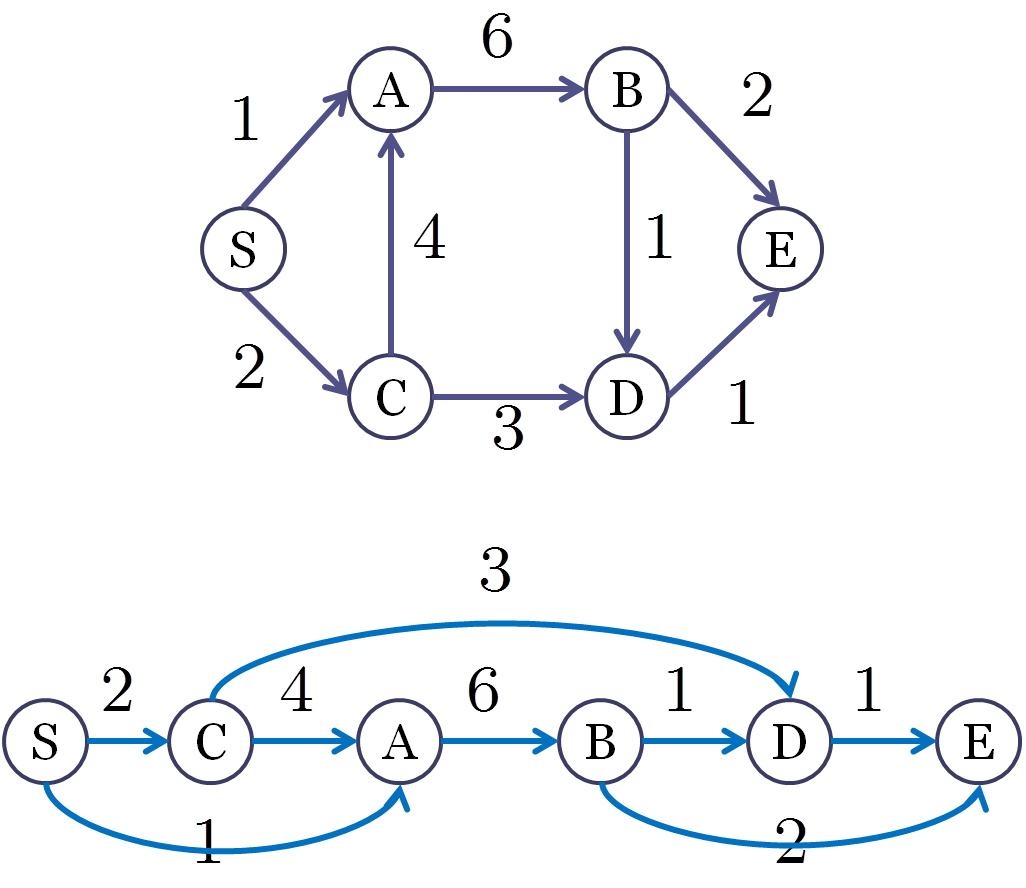
\includegraphics[scale=0.30]{figure/bfs_dfs/daglinear}
      \caption{{\scriptsize A dag and its topological sorting.}}
      \label{fig:daglinear}
    \end{center}
  \end{figure}

  \[
    dist(D) = \min \lbrace dist(B)+1, dist(C)+3 \rbrace.
  \]

\end{frame}


\begin{frame}
  \frametitle{Shortest paths}

  \textcolor{purple}{Shortest path without negative edges : \emph{Dijkstra algorithm}}

  \begin{figure}
    \begin{center}
      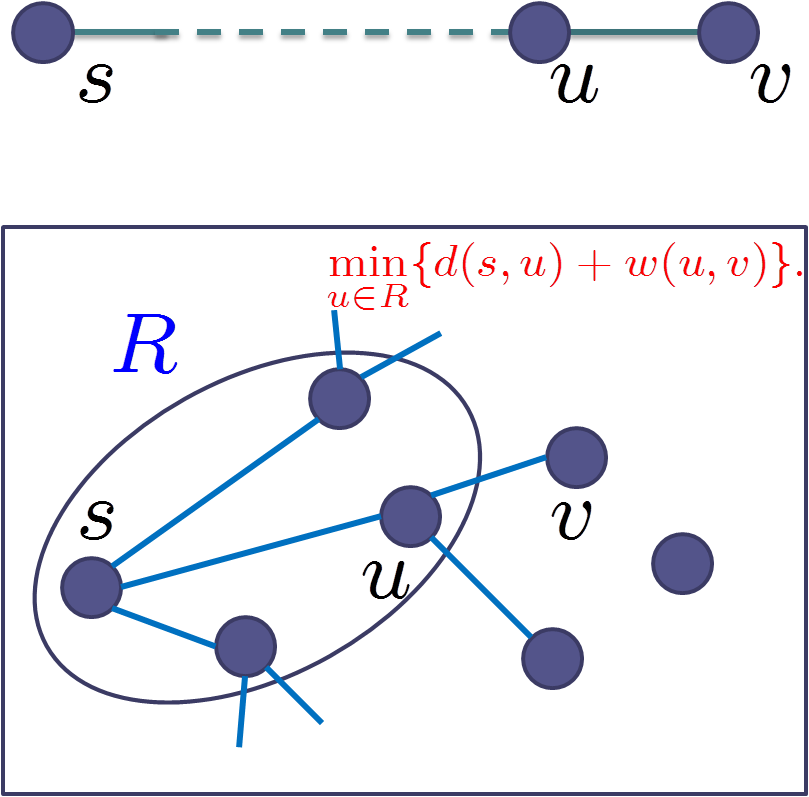
\includegraphics[scale=0.40]{figure/bfs_dfs/dijkstra}
      \caption{{\scriptsize Property of shortest paths.}}
      \label{fig:dijkstra}
    \end{center}
  \end{figure}

\end{frame}


\begin{frame}
  \frametitle{Priority queue implementations}

  \textcolor{purple}{Complexity of Dijkstra algorithm:}
  \begin{enumerate}
    \item makequeue, $\lvert V \rvert \cdot insert$
    \item $\lvert V \rvert \cdot deletemin$
    \item $\lvert E \rvert \cdot descreaseKey$
  \end{enumerate}

  \pause
  \vspace{0.50cm}

  \textcolor{purple}{Different implementations of priority queue:}

  {\scriptsize

    \begin{tabular}{|c||c|c|c|}
      \hline
      Implementation     & deletemin        & insert, decreaseKey       & total                 \\ \hline \hline
      Array              & $O(V)$           & $O(1)$                    & $O(V^2)$              \\ \hline
      Binary heap        & $O(\log{V})$     & $O(\log{V})$              & $O((V+E) \log {V})$   \\ \hline
      Fibonacci heap     & $O(\log{V})$     & $O(1)$                    & O$(V \log {V} + E)$   \\
      \hline
    \end{tabular}
  }

\end{frame}


\begin{frame}
  \frametitle{Shortest path with negative edges: \emph{Bellman-Ford algorithm}}

  \begin{figure}
    \begin{center}
      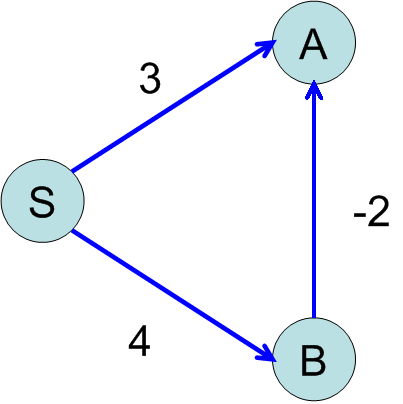
\includegraphics[scale=0.40]{figure/bfs_dfs/dijkstranegative}
      \caption{{\scriptsize Dijkstra algorithm fails if there are negative edges ([\textcolor{blue}{$P_{418}$ 8.14}]).}}
      \label{fig:dijkstranegative}
    \end{center}
  \end{figure}

\end{frame}



\begin{frame}
  \frametitle{All pairs of shortest paths: \emph{Floyd-Warshall algorithm}}

  \begin{figure}
    \begin{center}
      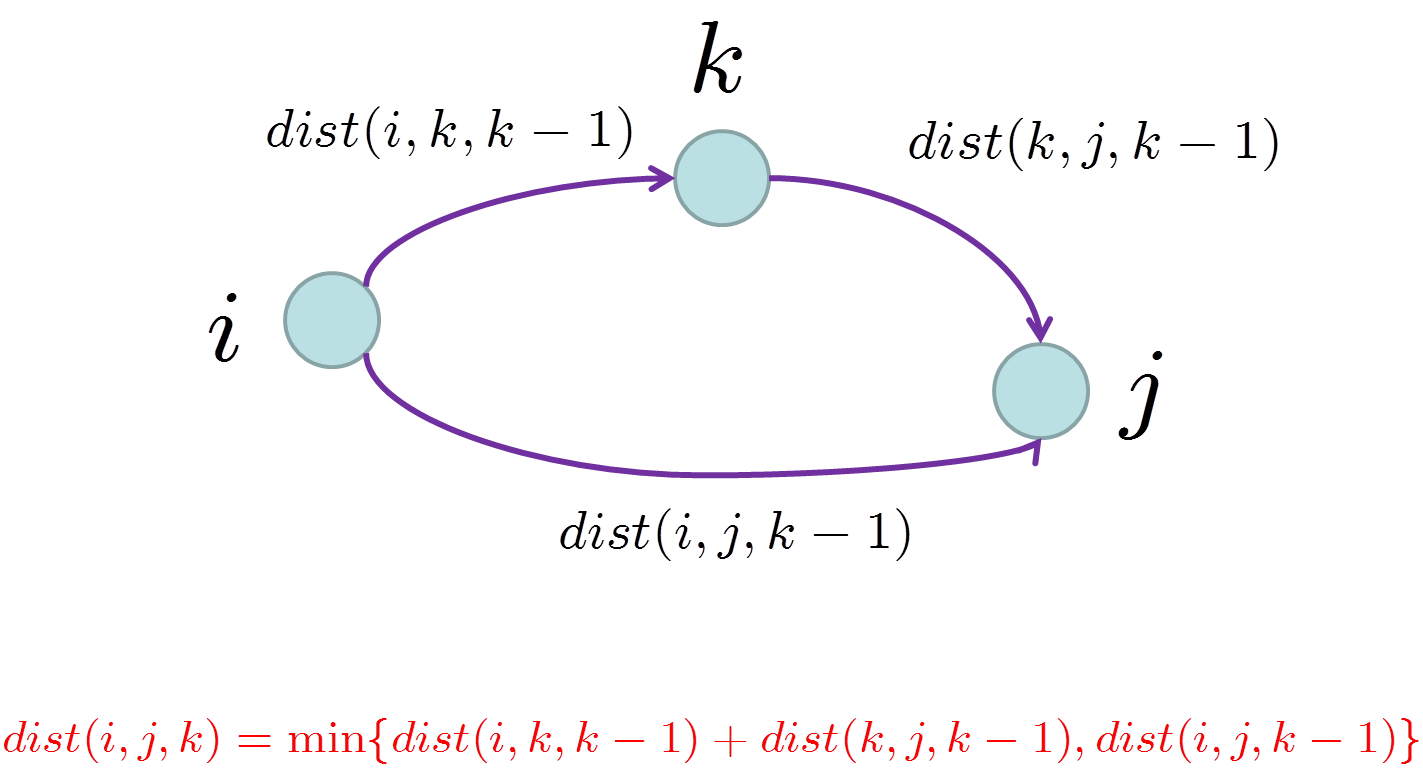
\includegraphics[scale=0.40]{figure/bfs_dfs/warshall}
      \label{fig:warshall}
    \end{center}
  \end{figure}

  \pause
  \vspace{0.40cm}
  \textcolor{red}{Assumption: No negative cycles.}

\end{frame}


\begin{frame}
  \frametitle{All pairs of shortest paths: \emph{Floyd-Warshall algorithm}}

  \begin{itemize}
    \item Routing table for all-pair shortest path ([\textcolor{blue}{$P_{448}$ 9.10}]).
    \item Length of shortest cycle in digraph ([\textcolor{blue}{$P_{448}$ 9.12}]).
  \end{itemize}

\end{frame}



\begin{frame}
  \frametitle{All pairs of shortest paths: \emph{Floyd-Warshall algorithm}}

  \begin{itemize}
    \item Routing table for all-pair shortest path ([\textcolor{blue}{$P_{448}$ 9.10}]).
    \vspace{0.50cm}

      \begin{figure}
        \begin{center}
          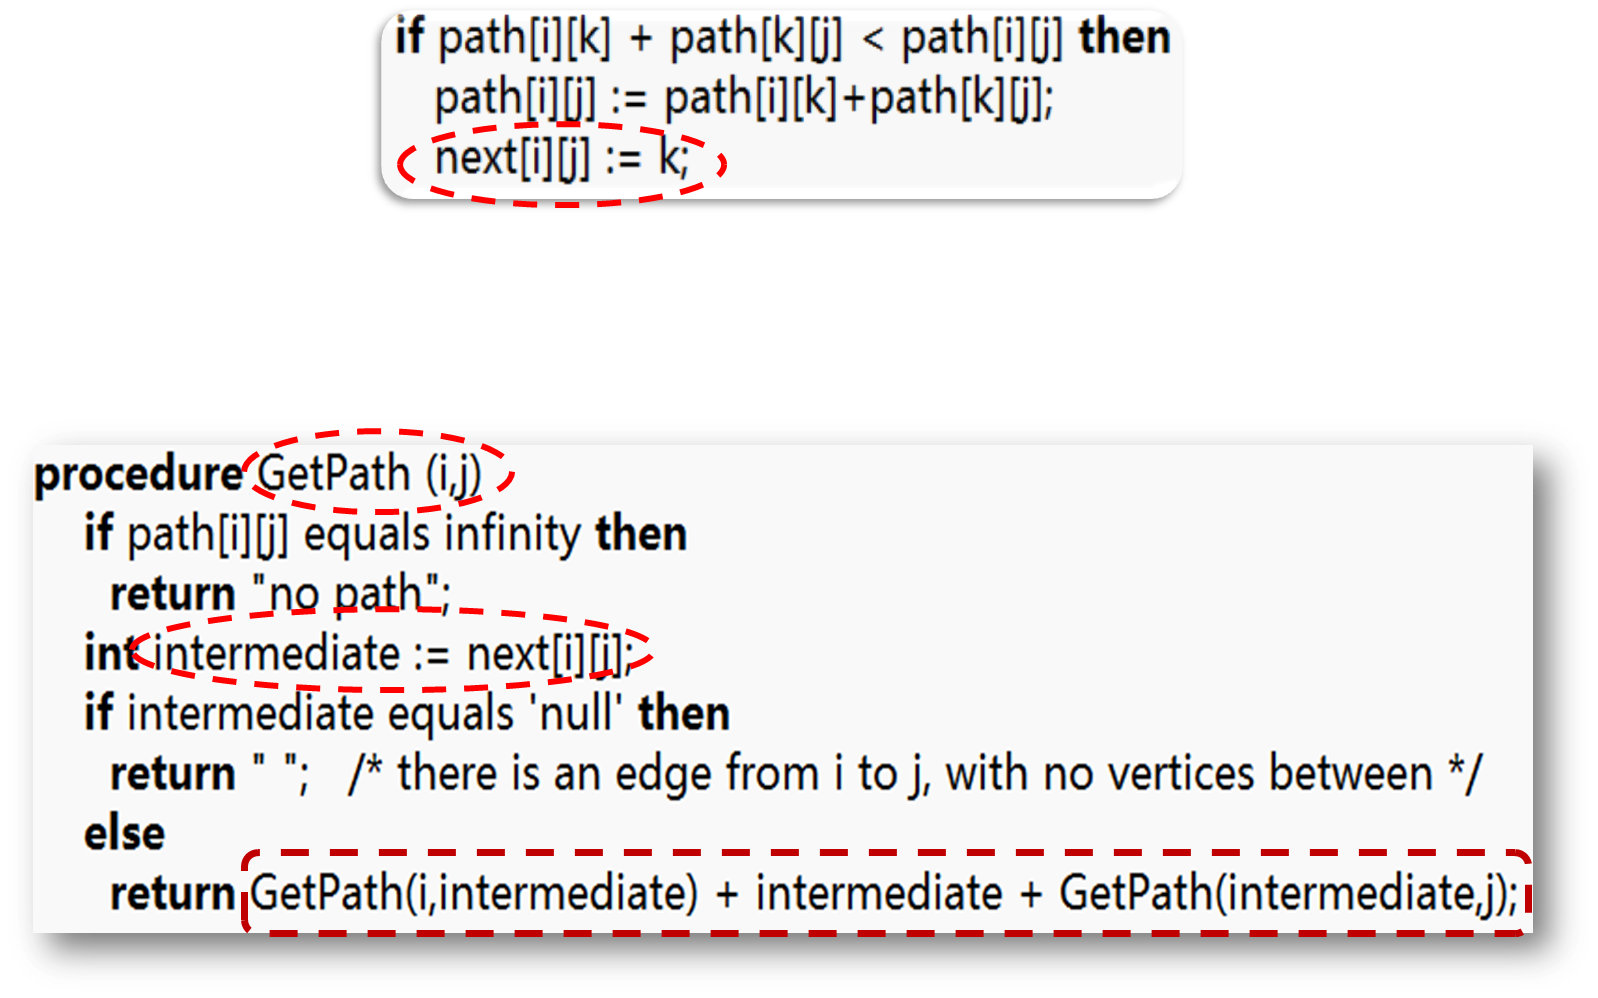
\includegraphics[scale=0.35]{figure/shortest_paths/route0}
          \caption{{\scriptsize Construction of routing table.}}
          \label{fig:route0}
        \end{center}
      \end{figure}
    \end{itemize}

\end{frame}



\begin{frame}
  \frametitle{All pairs of shortest paths: \emph{Floyd-Warshall algorithm}}

  \begin{itemize}
    \item Length of shortest cycle in digraph ([\textcolor{blue}{$P_{448}$ 9.12}]).
    \[
      path \lbrack i \rbrack \lbrack i \rbrack
    \]
    \[
      path \lbrack i \rbrack \lbrack i \rbrack < 0 ?
    \]
    \textcolor{red}{Fail for undirected graph:}
    \[
      \lbrace v, w \rbrace \to (v,w,v).
    \]
  \end{itemize}

\end{frame}


\begin{frame}
  \begin{figure}
    \begin{center}
      
\includegraphics[scale=0.60]{figure/thank}
      \label{fig:thank}
    \end{center}
  \end{figure}
\end{frame} 